% !TEX encoding = UTF-8 Unicode
\documentclass{article}

\usepackage{polski}
\usepackage[utf8]{inputenc}
\usepackage{subfig}
\usepackage{graphicx}
\usepackage{hyperref}
\usepackage[a4paper, left=2.5cm, right=2.5cm, top=3.5cm, bottom=2.5cm, headsep=2.5cm]{geometry}

\linespread{1.3}
\begin{document}
	
	\begin{titlepage}
		\centering
		{\scshape\LARGE Politechnika Wrocławska \par}
		{\scshape\Large Katedra Systemów i Sieci Komputerowych \par}
		
		\vspace{1cm}
		{\scshape\Large Technologie Sieciowe 2\par}
		\vspace{5cm}
		{\huge\bfseries Projekt przedmiotowy\par}
		\vspace{5cm}
		{\Large\itshape Magdalena Biernat, 225934\par}
		{\Large\itshape Michał Duński, 226081\par}
		\vfill
		Opiekun\par
		dr inż. Michał Kucharzak 
		
		\vfill
		{\large \today\par}
	\end{titlepage}
	\newpage
	\section{Wstęp}
	 Zadaniem tego projektu jest zaprojektowanie sieci komputerowej dla firmy RoboNet - przedsiębiorstwa zajmującego się produkcją oprogramowania dla specjalistycznych urządzeń ‒ robotów. Firma zatrudnia ok. 180 osób podzielonych na 3 grupy robocze, które zajmują 2 budynki. Budynek A posiada 3 kondygnacje, Budynek B posiada 1 kondygnację. Laboratorium znajduje się na parterze w budynku A. Sieć laboratoryjna nie ma dostępu do internetu. Do sieci laboratoryjnej mają dostęp wyłącznie Programiści i Testerzy. Serwery plików, www i pocztowy znajdują się w Budynku A i mieszczą się na dwóch kondygnacjach. Jeden serwer jest umieszczony w Budynku B.\newline
	 \noindent
	 \newline
Planujemy zastosować odpowiednie programy antywirusowe dla bezpieczeństwa oprogramowania oraz aby ograniczyć dostęp do sieci.
\newline
\noindent
\newline
	Projektowana sieć powinna cechować się jakością, niezawodnością oraz skalowalnością w przypadku potrzeby zwiększenia ilości pracowników w firmie. Ważnym czynnikiem jest również estetyczna jakość wykonania instalacji.
\newpage
\section{Inwentaryzacja zasobów: sprzętu, aplikacji, zasobów ludzkich}
Siedziba firmy mieści się w dwóch budynkach o oznaczeniach A i B. Budynek A jest trzypiętrowy, a budynek B ma tylko parter. 
\subsection{Wykaz pomieszczeń w budynkach}
\begin{enumerate}
	\item Budynek A
	\begin{itemize}
		\item Parter: administratorzy, serwerownia 1, laboratorium, recepcja
		\item Piętro 1: programiści i testerzy, serwerownia pocztowa, serwerownia www, toaleta
		\item Piętro 2: zarząd i kadry, programiści i testerzy, toaleta
	\end{itemize}
	\item Budynek B
		\begin{itemize}
		\item Parter: zarząd i kadry, programiści i testerzy, serwerownia 2, dwie toalety, recepcja
	\end{itemize}
\end{enumerate}
\subsection{Sprzęt}
Firma na wyposażeniu posiada:
\begin{itemize}
	\item 16 robotów
	\item 7 drukarek
	\item 24 kamery IP
\end{itemize}
\begin{tabular}{|c|c|c|c|c|}\hline
	\centering
	& Budynek A & Budynek A & Budynek A & 	Budynek B 	\\
	\centering
 & parter & piętro I & pietro II & parter \\
 \hline
drukarki & 1 & 2 & 2 & 2\\
\hline
roboty (urządzenia) & 16 & - & - & - \\
\hline
kamery IP & 8 & 4 & 4 & 8 \\
\hline
\end{tabular}
\newpage
\section{Analiza potrzeb użytkowników – wymagania zamawiającego}
\subsection{Dostęp do Internetu}
Na podstawie bieżących potrzeb firmy RoboNet(tabela niżej), przy uwzględnieniu ewentualnego rozrostu przedsiębiorstwa oraz obecnych na rynku ofert najlepszym rozwiązaniem w kwestii dostępu do Internetu jest łącze symetryczne 100Mb/100Mb.\newline
W tabeli sumowane są wartości przepływów z i do Internetu dla każdego użytkownika. Wartości są w kb/s.
\newline
\begin{tabular}{|c|c|c|} \hline
	& down & up \\
	\hline
	serwer www & 7 680 & 16 320\\
	serwer pocztowy & 10 680 & 4 920\\
	wideorozmowy & 7 040 & 7 040 \\
	komunikator & 9 600 & 9 600 \\
	praca w chmurze & 6 664 & 10 472 \\
	przeglądarka & 24 920 & 5 020 \\
	\hline
	\hline
	SUMA & 66 584 & 53 372\\
\hline
\end{tabular}
\subsection{Sieć lokalna}
W celu zapewnienia wystarczającej przepustowości w sieci lokalnej wykorzystane będzie okablowanie w technologii 100Base-TXFast Ethernet(okablowanie poziome) oraz 1000Base-T Gigabit Ethernet(okablowanie pionowe).  Wymagana przepustowość sieci lokalnej została podana w tabeli poniżej. Wartości zostały sumowane dla przepływów lokalnych dla każdego użytkownika. Wartości są w kb/s.
\newline
\begin{tabular}{|c|c|c|} \hline
	& down & up \\
	\hline
	serwer pliów 1 & 34 400 & 69 600\\
	serwer plików 2 & 123 600 & 98 000\\
	serwer www & 35 400 & 5 940\\
	serwer pocztowy & 67 000 & 77 520\\
	drukarki & 1 800 & 30 900\\
	roboty & 27 200 & 27 200\\
	\hline
	\hline
	SUMA & 289 400 & 309 160\\
	\hline
\end{tabular}
\newpage
\section{Założenia projektowe}
Projekt zakłada stworzenie sieci dla przedsiębiorstwa zajmującego się produkcją oprogramowania dla specjalistycznych urządzeń ‒ robotów, których zastosowanie jest ściśle tajne. Przedsiębiorstwo posiada dwa budynki. W jednym pracuje 100 użytkowników (komputerów), 5 drukarek, 16 kamer IP, 16 robotów i 3 serwery. W drugim pracuje 80 użytkowników (komputerów, 2 drukarki, 8 kamer IP i 1 serwer. W każdym budynku projekt zakłada sieć WiFi dla 150 gości. Budynek A ma trzy kondygnacje, budynek B posiada tylko parter. Przed stworzeniem sieci komputerowej zostanie wykonane (we wcześniejszym terminie i dla odpowiednich pomieszczeń) dostosowanie instalacji elektrycznej.
W obu budynkach będą znajdować się przełączniki warstwy trzeciej.
Dla połączenia z Internetem zostaną zamontowany router chroniony firewallem.
Z sieci gości możliwy jest wyłącznie dostęp do Internetu.
Wszyscy pracownicy mają dostęp do wszystkich drukarek i pozostałych serwerów. Z Internetu możliwy jest dostęp wyłącznie do Serwera WWW i Serwera Pocztowego.
Okablowanie poziome w technologii 100Base-TXFast, okablowanie pionowe w technologii 1000Base-T Gigabit Ethernet oraz połączenie światłowodowe między budynkami. Dla zachowania odpowiedniej estetyki kable zostaną schowane w podłodze lub podwieszanym suficie.
Zastosowanie odpowiednich programów antywirusowych dla bezpieczeństwa oprogramowania oraz ograniczony dostęp do sieci.

\newpage
\section{Projekt sieci}
\subsection{Projekt logiczny wraz z opisem koncepcji rozwiązania i uzasadnieniem}
\begin{figure}[!ht]	
	\centering
	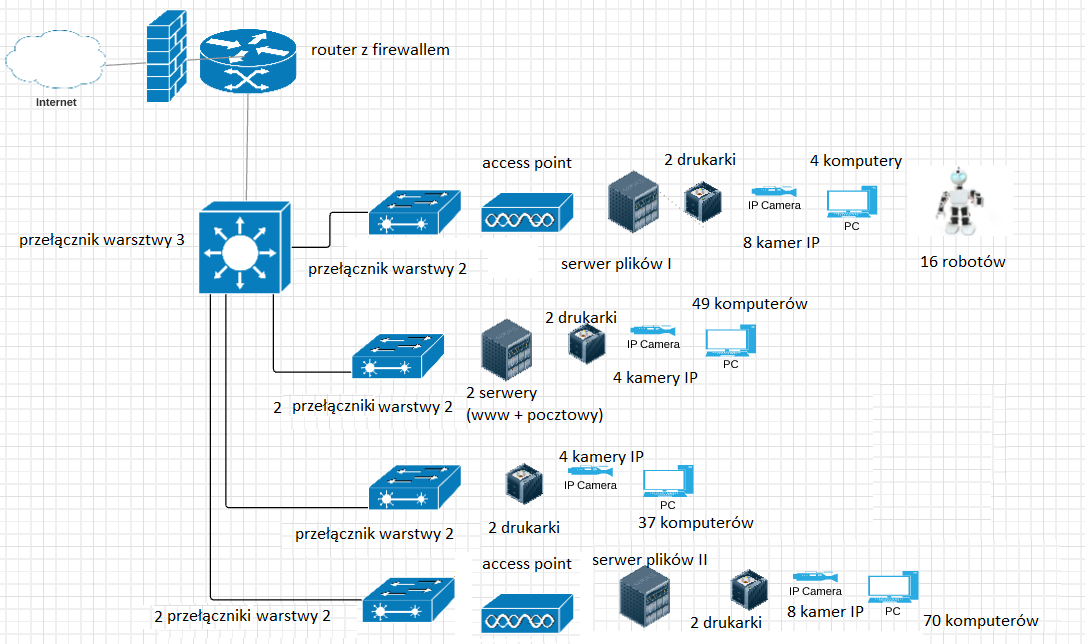
\includegraphics[height=10cm]{projekt_logiczny2.png}
	\caption{Schemat zamka szyfrowego}
	\label{fig:obrazek 1}
\end{figure}
Dostęp do internetu jest przez router z firewallem. Przełącznik warstwy 3 łączy przełączniki warstwy 2. Każde piętro ma przełącznik lub dwa (zależy od liczby potrzebnych wejść).

\subsection{Wybór urządzeń}
\begin{enumerate}
	\item Przełącznik warstwy 3\newline
	\href{https://www.cisco.com/c/en/us/products/collateral/switches/sge2000-24-port-gigabit-switch/data\_sheet\_c78-502447.html}{Cisco SGE2000}
	\begin{itemize}
		\item 24 porty RJ-45 10BASE-T/100BASE-TX/1000BASE-T
		\item Port konsolowy
		\item Port RPS do podłączenia zapasowego źródła zasilania
	\end{itemize}
	
	
	
	
	\item Przełącznik warstwy 2 - 48 portów
	\href{https://www.cisco.com/c/en/us/products/collateral/switches/slm248p-48-port-10-100-2-port-gigabit-smart-switch-sfps-poe/data_sheet_c78-501235.html}{Cisco SLM248P}
	\begin{itemize}
		\item 48 portów RJ-45 10BASE-T/100BASE-TX/1000BASE-T
		\item 2 porty SFP combo
		\item Wbudowany interfejs WWW
	\end{itemize}
	\item Router
	\href{ https://www.cisco.com/c/en/us/products/collateral/routers/rv325-dual-gigabit-wan-vpn-router/datasheet-c78-729726.html}{Cisco RV325-K9-G5}
	\begin{itemize}
		\item 2 porty RJ-45 WAN
		\item Obsługa VPN
	\end{itemize}
	
	\item Serwer
\href{ https://www.cisco.com/c/en/us/products/collateral/servers-unified-computing/ucs-c-series-rack-servers/datasheet-c78-739281.html}{Cisco UCS C220 M5 Rack Server}
	
	
	\item Access Point
	\href{ https://www.cisco.com/c/en/us/products/collateral/wireless/aironet-1850-series-access-points/datasheet-c78-734256.html}{Cisco Aironet 1850 Series}
	
	\begin{itemize}
		\item Agregacja pakietów A-MPDU (Tx/Rx), A-MSDU (Tx/Rx)
		\item Kanały 20 i 40 MHz
		\item Liczba nienakładających się kanałów
		\begin{itemize}
			\item 2.4GHz
			\begin{itemize}
			\item 802.11b/g - 3
			\item 802.11n - 3
			\end{itemize}
			\item 5GHz
			\begin{itemize}
				\item 802.11a 
			\end{itemize}
		\item 20 MHz - 25
		\begin{itemize}
			\item 802.11n
		\end{itemize}
		\item 20 MHz - 25
		\item 40 MHz - 12
		\begin{itemize}
			\item 802.11ac
		\end{itemize}
		\item 20 MHz - 21
		\item 40 MHz - 12
		\item 80 MHz - 6
		\end{itemize}
	\end{itemize}

	
	
	
\end{enumerate}

\end{document}